% Requires: \usepackage{booktabs,graphicx}
\subsection{Same-Dimension Comparison on OpenML}
\label{subsec:openml-supcon}

We next compare KDMLP, feature-level SupCon~\cite{khosla2020supervised}, and KFDA
on 13 OpenML tasks: breast-cancer (13), breast-w (15), credit-g (31), segment
(36), diabetes (37), sonar (40), splice (46), heart-statlog (53), hypothyroid
(57), waveform-5000 (60), banana (1460), ringnorm (1496), and Titanic (40945).
Multiclass datasets are converted to one-versus-rest binary tasks.  Each dataset
uses a stratified $60\%/40\%$ train/test split and the common dimension grid
$r\in\{1,2,3,4,5,6,32,64\}$.

KDMLP searches its large- and small-mean regimes with linear, RBF, and Laplacian
Stage-1 kernels, followed by a training-validated SVM.  SupCon uses the same
feature-level architecture as in Section~\ref{subsec:gaussian-supcon}: its
$128$-dimensional encoder output is reduced by training-set PCA to dimension $r$
and evaluated by a training-validated logistic probe.  For binary KFDA, the
between-class scatter has rank at most one; consequently, KFDA supplies one
nonzero discriminant direction and its accuracy is repeated across $r$ as a flat
reference.

\begin{table}[t]
\centering
\caption{Mean test accuracy across the 13 OpenML tasks.}
\label{tab:openml-supcon-same-r}
\small
\begin{tabular}{c c c c}
\toprule
$r$ & Best KDMLP & SupCon & KFDA \\
\midrule
1  & \textbf{0.8655} & 0.8156 & 0.8368 \\
2  & \textbf{0.8668} & 0.8302 & 0.8368 \\
3  & \textbf{0.8665} & 0.8463 & 0.8368 \\
4  & \textbf{0.8627} & 0.8550 & 0.8368 \\
5  & \textbf{0.8698} & 0.8580 & 0.8368 \\
6  & 0.8638 & \textbf{0.8639} & 0.8368 \\
32 & \textbf{0.8780} & 0.8617 & 0.8368 \\
64 & \textbf{0.8716} & 0.8583 & 0.8368 \\
\bottomrule
\end{tabular}
\end{table}

At $r=32$, KDMLP obtains the largest mean accuracy, exceeding SupCon by $0.0162$
and KFDA by $0.0412$.  At this dimension KDMLP wins/ties/loses against SupCon on
$6/3/4$ datasets; at $r=64$ the corresponding count is $10/0/3$.  The individual
curves show that the effect of $r$ is dataset dependent: banana improves steadily,
sonar peaks at $r=32$, hypothyroid is strongest at $r=1$, and ringnorm remains
near its ceiling throughout the grid.

\begin{figure}[t]
\centering
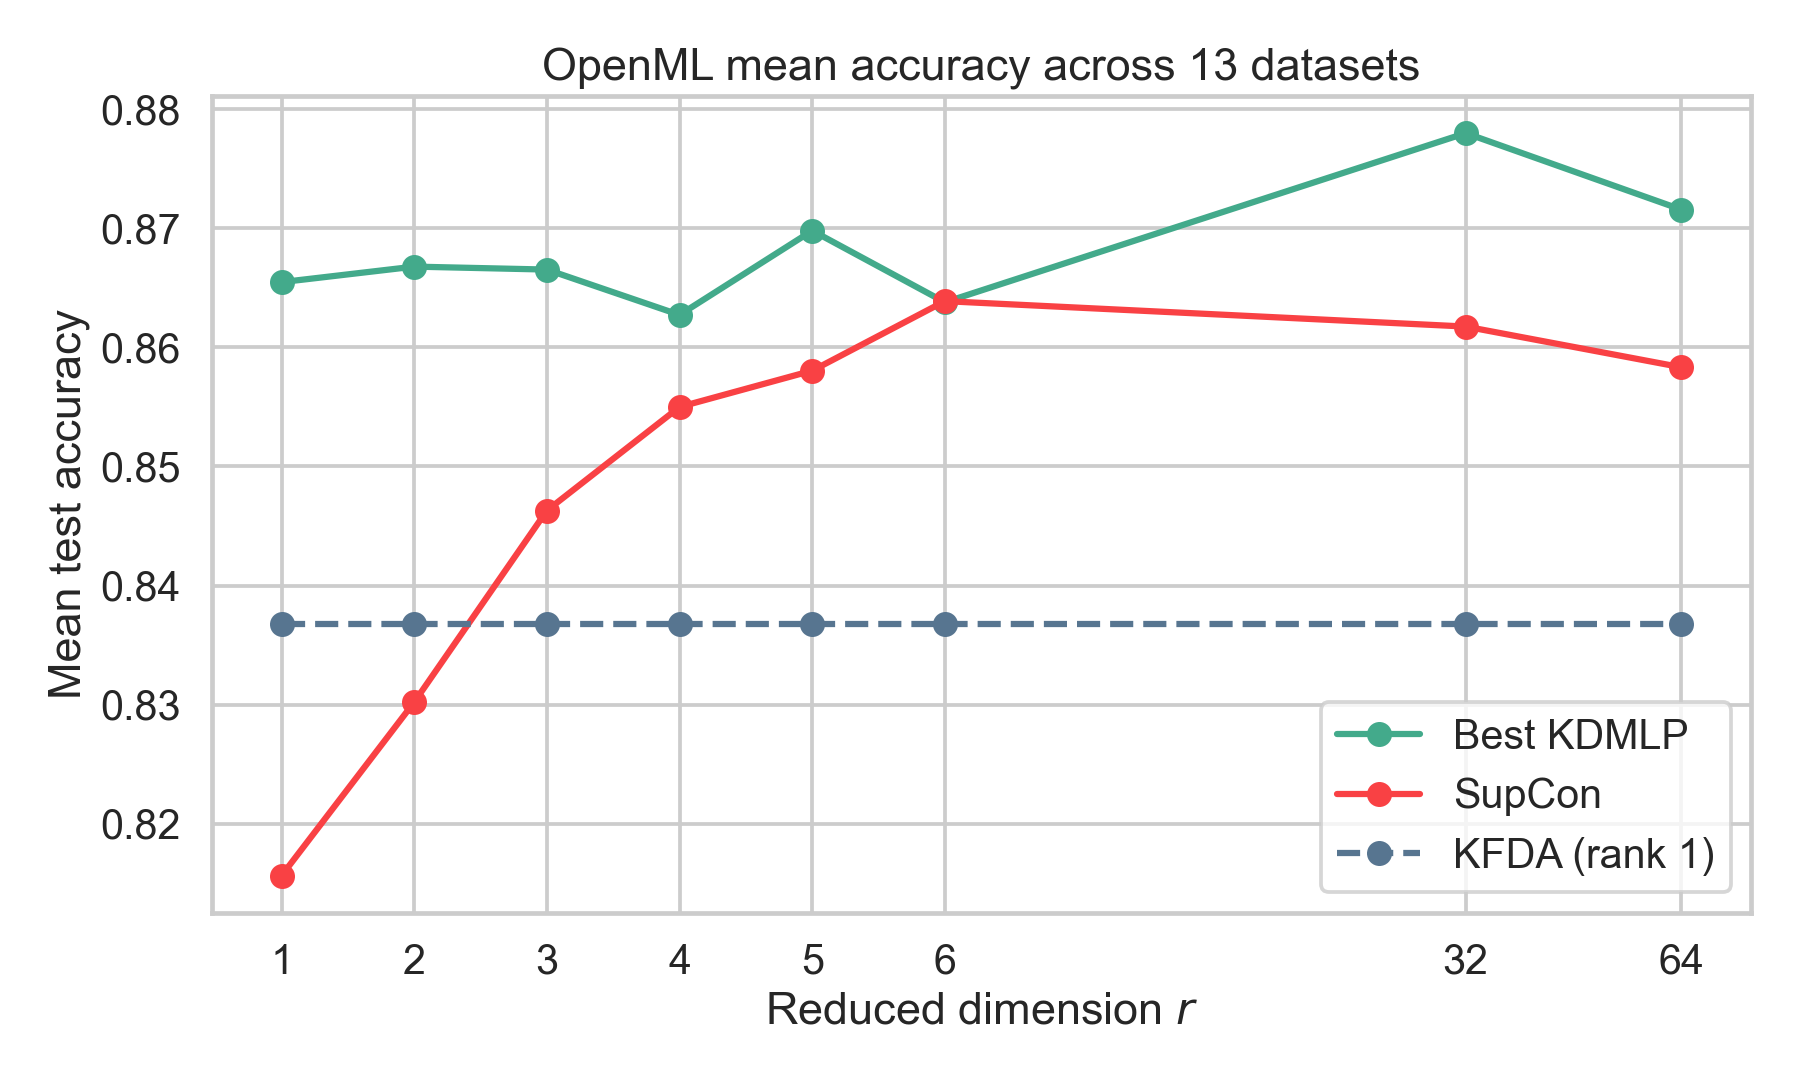
\includegraphics[width=0.82\linewidth]{simulations/supcon_openml_workspace/outputs_same_r/openml_same_r_mean_curve.png}
\caption{Mean same-$r$ accuracy across the 13 OpenML tasks.}
\label{fig:openml-supcon-mean}
\end{figure}

\begin{figure*}[t]
\centering
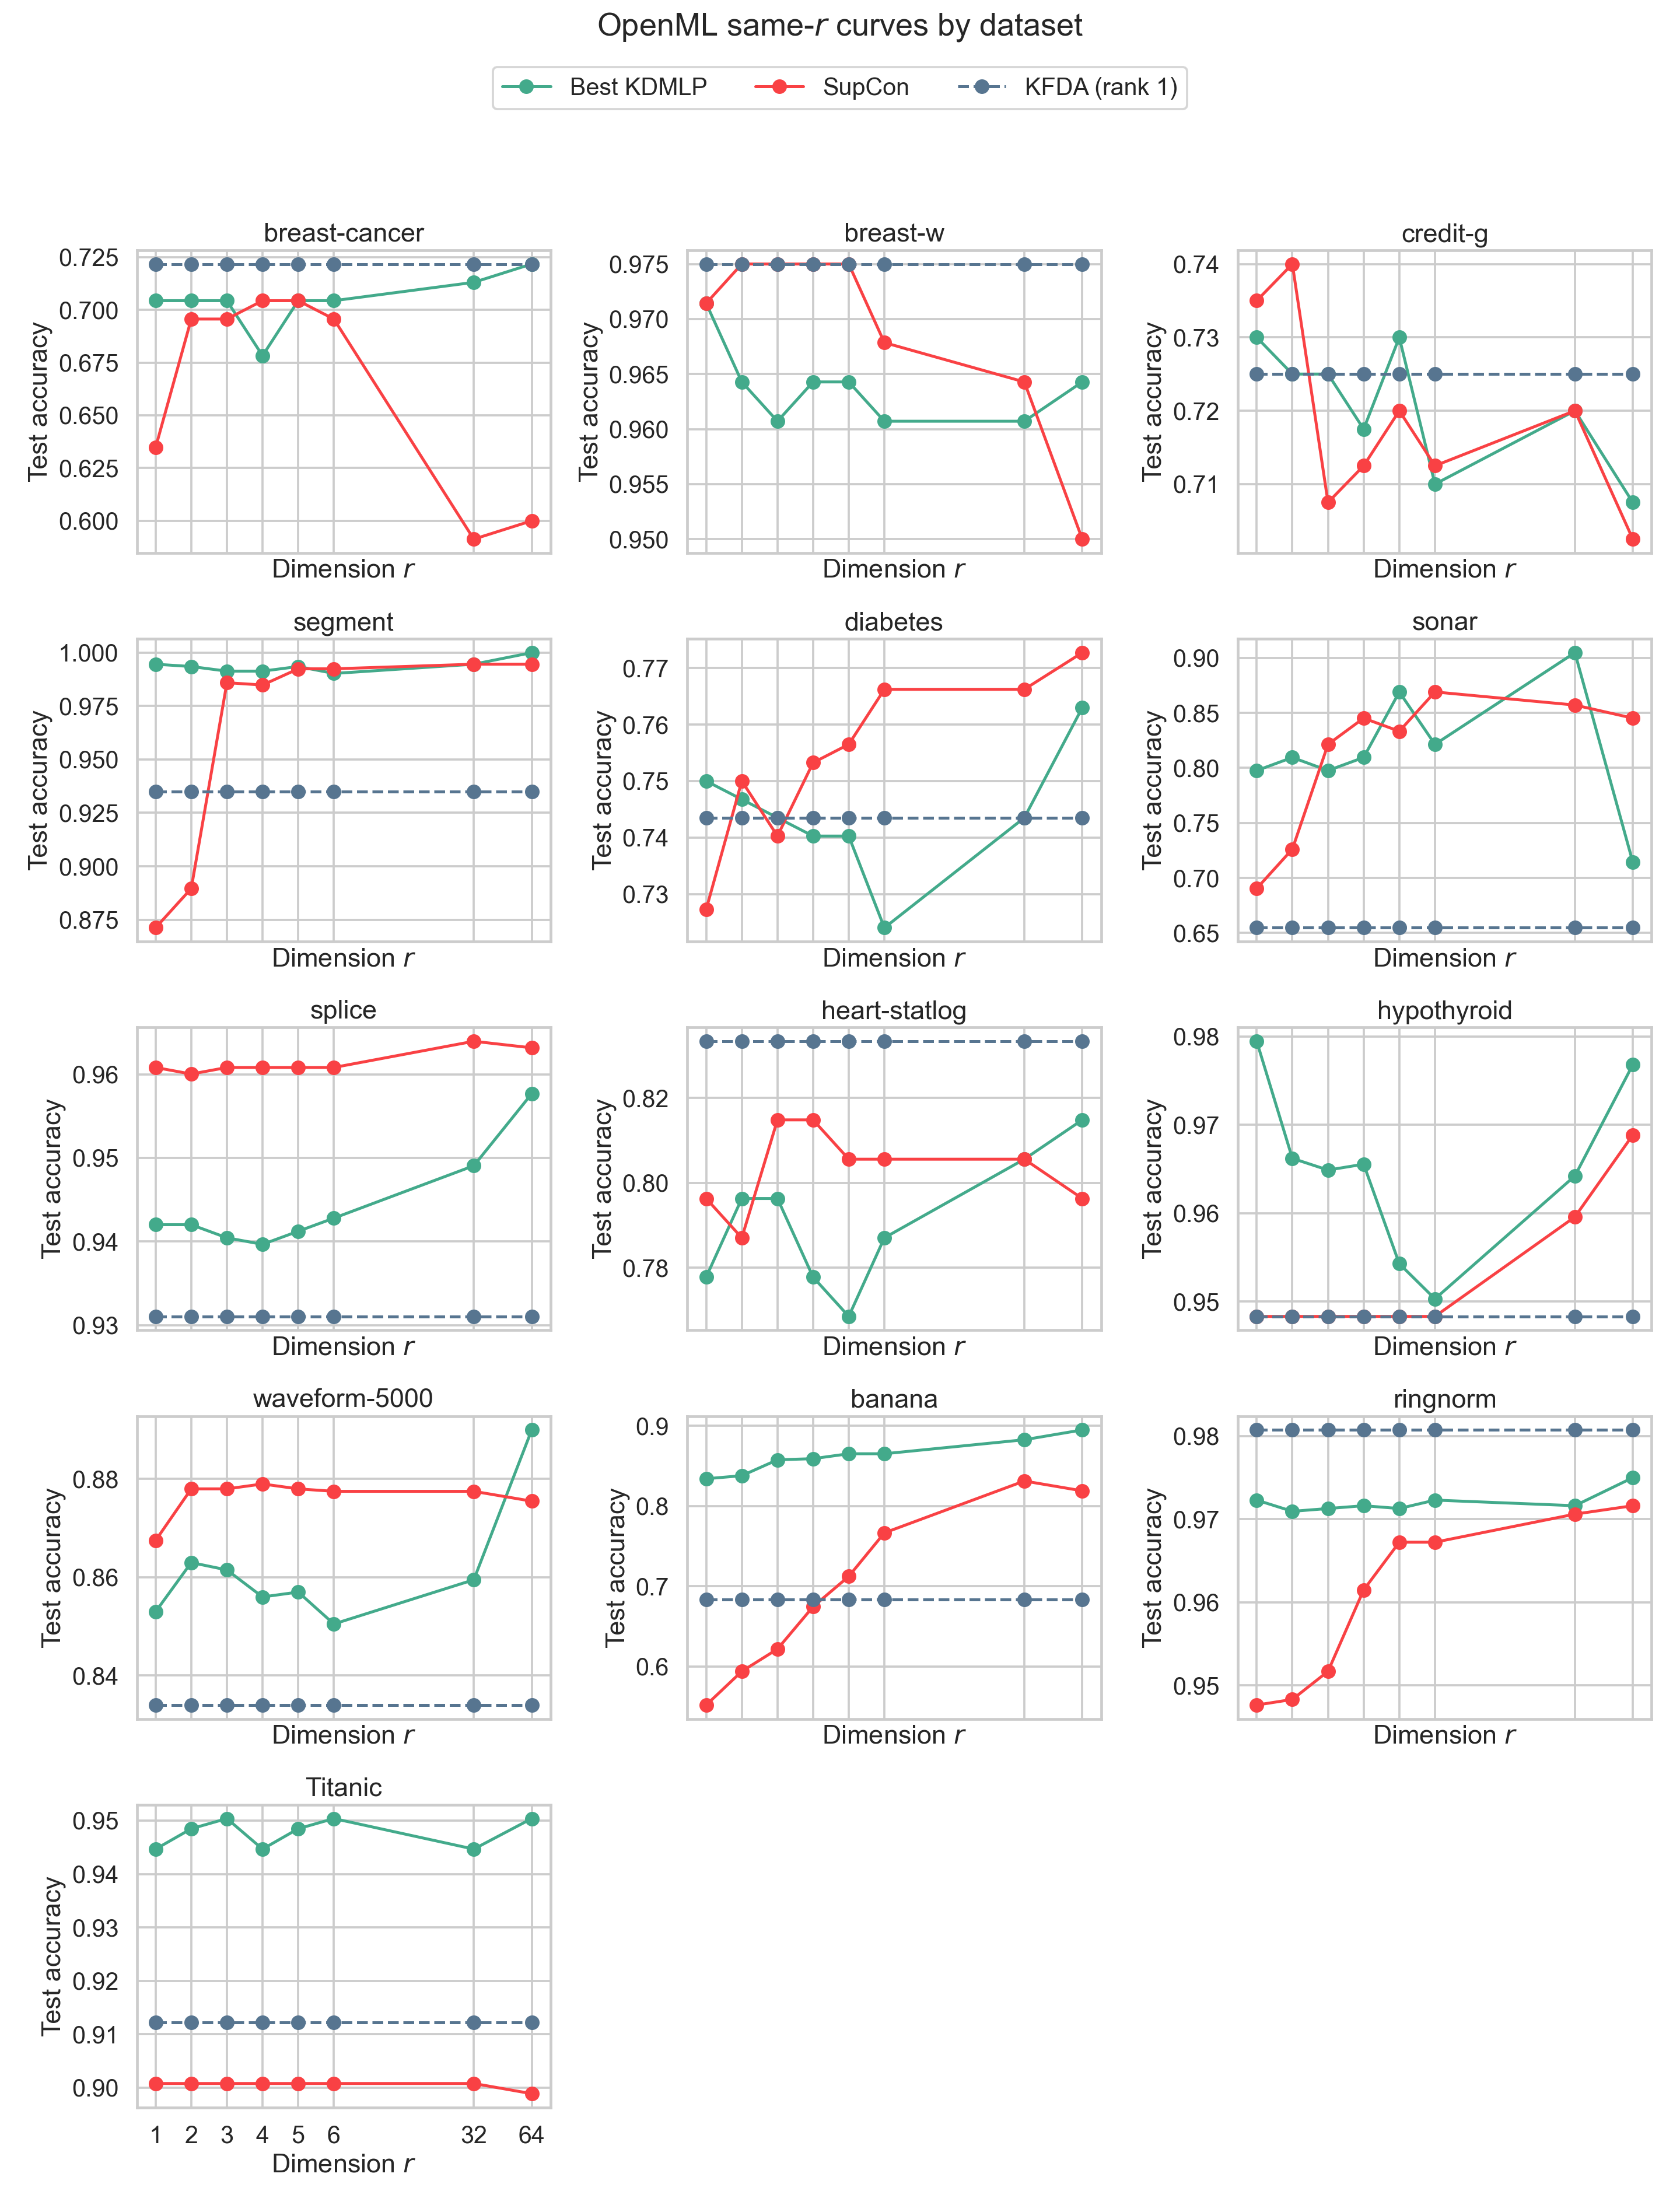
\includegraphics[width=0.94\textwidth]{simulations/supcon_openml_workspace/outputs_same_r/openml_all_same_r_curves.png}
\caption{Dataset-level same-$r$ curves for KDMLP, SupCon, and rank-one KFDA.}
\label{fig:openml-supcon-all}
\end{figure*}

This experiment is an exploratory dimension-sensitivity study rather than a
fully nested benchmark.  The saved run uses one split, fits unsupervised tabular
preprocessing before that split, and retrospectively selects the best KDMLP
kernel/regime at each $r$ by test accuracy; moreover, KDMLP/KFDA and SupCon use
different downstream probes.  Therefore, the reported values are descriptive.
A confirmatory evaluation should fit preprocessing on each training fold, use
repeated outer splits, select all models within nested validation, and use a
common downstream classifier.
